\documentclass[10pt,twocolumn]{article}
\usepackage[margin=1.7cm,columnsep=0.55cm]{geometry}
\usepackage{amsmath,amssymb,graphicx,booktabs,microtype}
\usepackage[hidelinks]{hyperref}
\usepackage[small,compact]{titlesec}
\setlength{\parskip}{1pt}
\setlength{\textfloatsep}{7pt}
\setlength{\floatsep}{6pt}

\title{\vspace{-7mm}\large\bf Horizon-Gated JEPA: Label-Free Separation of\\
Slow and Fast Factors in Time Series}
\author{Jaechan Lee}
\date{July 25, 2026 --- compact progress report (extended version available)}

\begin{document}
\maketitle
\vspace{-9mm}

\section{Motivation and claim}
Practitioners want the \emph{slowly-varying state} of a time series (machine
health, diagnosis, activity) \emph{separated} from fast variation (vibration,
beat morphology, gait), not merely co-encoded: separation is what enables
selective domain robustness and interpretable state trajectories. Frequency
decomposition \cite{mallat1999wavelet,huang1998empirical} fails in principle
--- a slow factor need not live in a low band (bearing health rides the
envelope of high-frequency resonance \cite{randall2011rolling}); sequential
VAEs (DSAE \cite{hsu2017unsupervised}, C-DSVAE \cite{bai2021contrastively})
separate only \emph{static} content via fragile reconstruction; and
horizon-conditioned JEPAs (HEPA \cite{hepa2026}) encode multi-scale dynamics
without factoring them.

Our observation: \textbf{the prediction horizon --- free in any predictive
learner --- is itself a supervision axis}, because only slow information
helps predict the far future
\cite{bialek2001predictability,creutzig2009past}. \emph{H1: gating a latent
block out of the predictor at long horizons concentrates slow factors in the
ungated block, with no labels.} Two refinements set the claim's exact
strength. \emph{H2 (assignment asymmetry):} the gate \emph{assigns} slow
information (provable); \emph{exclusion} of fast information rests on a
narrow bottleneck plus a decorrelation penalty. \emph{H3:} the gate requires
\emph{latent} targets; raw-signal prediction smears detail everywhere. Unlike
slow feature analysis \cite{wiskott2002slow} we select by predictive value,
not trajectory slowness; unlike temporal nonlinear-ICA
(TCL \cite{hyvarinen2016unsupervised}, SlowVAE \cite{klindt2021towards}) we
have no full identifiability theorem --- our inductive bias, in the sense
required by \cite{locatello2019challenging}, is the timescale gap itself.

\begin{figure}[t]
\centering
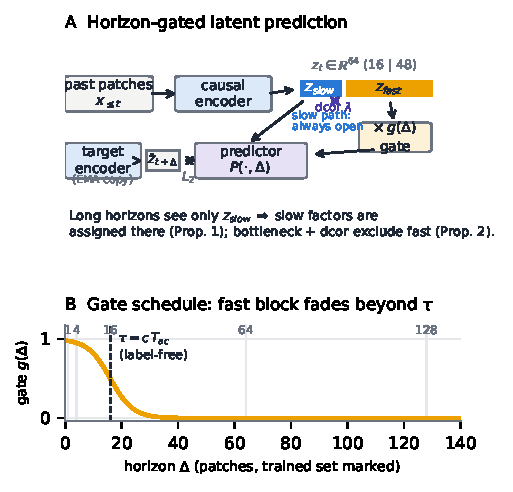
\includegraphics[width=.96\linewidth]{fig_method.pdf}
\vspace{-4mm}
\caption{\small \textbf{Method.} \textbf{A:} the encoder splits each embedding
into a narrow slow block and a wide fast block; the slow path is always open,
the fast path is gated by $g(\Delta)$; dcor decorrelates blocks. \textbf{B:}
the gate closes beyond $\tau=c\,T_{\mathrm{ac}}$, set label-free from the
signal's autocorrelation time.}
\vspace{-3mm}
\end{figure}

\section{Method}
A causal transformer encoder ($\sim$0.5M params) maps patches to
$z_t=[z^{\mathrm{slow}}_t;z^{\mathrm{fast}}_t]\in\mathbb R^{64}$ (16 dims
slow). A predictor conditioned on $\Delta\in\{1,4,16,64,128\}$ patches
regresses the EMA target encoder's embedding (CPC multi-horizon predictor
\cite{oord2018representation} with I-JEPA-style targets
\cite{assran2023self,baevski2022data2vec}, as in HEPA \cite{hepa2026}; our
contribution is the gate, not the backbone):
\[
\mathcal L=\textstyle\sum_{\Delta}\big\|
P\big(z^{\mathrm{slow}}_t, g(\Delta)z^{\mathrm{fast}}_t, \Delta\big)
-\bar z_{t+\Delta}\big\|^2+\lambda\mathcal L_{\mathrm{dcor}},
\]
with soft gate $g(\Delta)=\sigma((\tau-\Delta)/w)$, where $\sigma$ is the
logistic sigmoid and $w$ (4 patches) sets the transition width, so the fast
block fades smoothly from open ($g{\approx}1$) to closed ($g{\approx}0$)
around $\tau$. The gate is asymmetric:
short horizons see both blocks (fast dynamics are conditioned on slow state).
$\mathcal L_{\mathrm{dcor}}$ penalizes squared cross-covariance
(VICReg-lineage \cite{bardes2022vicreg}). $\tau=c\,T_{\mathrm{ac}}$
($c{\approx}2.5$) comes from the signal's autocorrelation decay --- label-free,
and doubling as a pre-training applicability screen.

\section{Theory (proofs in extended report)}
\textbf{Prop.~1 (inclusion).} If the far future is conditionally independent
of the past given the slow state ($\Delta\ge\Delta_0$: the timescale gap) and
the gate is closed at some trained $\Delta^*\!\ge\!\Delta_0$, every population
minimizer makes $z^{\mathrm{slow}}$ mean-sufficient for the far future; with
affinely independent regime-conditional target means, the slow-state
posterior is a function of $z^{\mathrm{slow}}$. \emph{(Square-loss tower
decomposition.)}
\textbf{Prop.~2 (no exclusion).} For any minimizer, a Borel re-encoding
injects any fast statistic into $z^{\mathrm{slow}}$ at identical loss ---
exclusion is \emph{not identified} by the objective under any gate schedule;
dcor removes only linearly-readable duplication. So measured nonlinear leak
is the objective's boundary, not a bug; in practice exclusion comes from the
narrow block (continuous encoders cannot realize the pathological
injections). A TCL-style uniqueness theorem remains open.

\begin{figure}[t]
\centering
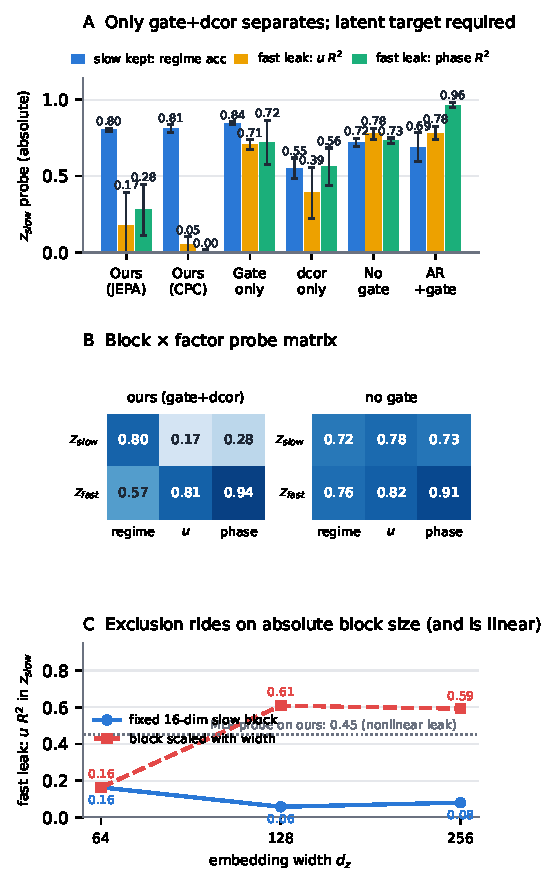
\includegraphics[width=.9\linewidth]{fig_mech.pdf}
\vspace{-4mm}
\caption{\small \textbf{Mechanism (synthetic, leak-free, 3 seeds).}
\textbf{A:} only gate+dcor separates; the latent-contrastive cell (CPC) is
best; raw-target (AR) fails. \textbf{B:} block$\times$factor matrices.
\textbf{C:} exclusion tracks \emph{absolute} block size (fixed 16-dim holds
at $d_z{=}256$); dotted line: nonlinear-probe leak (see limitations).}
\vspace{-3mm}
\end{figure}

\section{Experiments}
\textbf{Protocol.} Synthetic two-timescale oscillator (3-state Markov regime,
dwell 3000 steps, sets carrier frequency $\pm5\%$; fast OU factor, lifetime
50 steps; amplitudes equalized so no short-window statistic reveals the
regime). Real data: HAPT \cite{reyes2016transition} (subject split), PTB-XL
\cite{wagner2020ptb} (patient split), XJTU-SY \cite{wang2020xjtu} (bearing
split). Probes fit on train groups, tested on held-out groups over disjoint
windows; \emph{absolute} scores; RankMe \cite{garrido2023rankme} monitors
collapse; $n{=}3$ seeds, one backbone and budget for all variants. Results
are organized as findings F1--F5.

\textbf{F1 --- separation, and alternatives do not suffice (Tab.~1).}
Gate+dcor keeps the regime in $z^{\mathrm{slow}}$ (acc $0.80$ vs.\ full
$0.69$ --- selective-use payoff) while cutting fast leak to $0.19/0.27$
($0.79/0.73$ ungated). Label-free rotations of the \emph{ungated} embedding
(SFA/ICA/PCA) each trade one side away: separation is created by the
objective, not recoverable post hoc. A theory-bearing competitor also fails:
an architecture-matched SlowVAE \cite{klindt2021towards} never captures the
regime at all (slow block $0.63$, \emph{full} embedding $0.54$) ---
reconstruction is local, and a factor requiring integration over hundreds of
steps never enters its code.

\begin{table}[h]
\centering\small
\caption{\small Unmixing control (synthetic, 3 seeds): 16-dim ``slow''
subspace of the ungated embedding vs.\ our gate.}
\vspace{-1mm}
\begin{tabular}{@{}lccc@{}}
\toprule
Method & regime $\uparrow$ & $u$-leak $\downarrow$ & phase-leak $\downarrow$\\
\midrule
SFA (16 slowest) & 0.57 & 0.00 & 0.00 \\
ICA (16 slowest) & 0.52 & 0.12 & 0.17 \\
PCA (top 16)     & 0.76 & 0.80 & 0.91 \\
\textbf{gate+dcor (ours)} & \textbf{0.80} & \textbf{0.19} & \textbf{0.27}\\
\bottomrule
\end{tabular}
\vspace{-2mm}
\end{table}

\textbf{F2 --- latent targets, either objective.} The identical gate on
raw-patch (AR) prediction separates nothing (leak $\ge0.78$). On a latent
\emph{contrastive} objective (CPC-InfoNCE vs.\ EMA embeddings) it separates
\emph{best}: regime $0.81$, leak $0.05/0.00$, with $z^{\mathrm{fast}}$
retaining the fast factors ($0.85/0.95$; no collapse). The mechanism is
latent-target-family, not JEPA-specific.
\textbf{F3 --- gate assigns, penalty purifies (Prop.~2).} Gate-alone barely
reduces leak ($0.74/0.79$); dcor-alone degenerates (regime $0.55$); only the
combination works. Adding target-side removal pressure does not rescue
gate-alone.
\textbf{F4 --- exclusion rides on capacity, and scales.} Leak tracks the
\emph{absolute} slow-block size: a fixed 16-dim block holds when the backbone
widens to $d_z{=}128/256$ (leak $0.06/0.08$) while proportionally scaled
blocks let it flood back ($\approx0.6$) --- the mechanism transfers to wide
backbones provided the slow block stays narrow.
\textbf{F5 --- real data (Fig.~3, Tab.~2).} HAPT: leak $0.56\!\to\!0.17$ at
activity F1 $0.71$, holding on \emph{unseen subjects}; dcor \emph{hurts}
here. PTB-XL: dcor \emph{helps} (leak $0.61\!\to\!0.41$) --- its polarity is
data-dependent and not yet decidable label-free. XJTU is the predicted
negative: carrier and envelope share one timescale
($T_{\mathrm{ac}}\!\approx\!1$--$2$ patches), the gate correctly does
nothing; on the non-circular health target (lifetime fraction, held-out
bearings) every method is weak, classical envelope/low-pass features fail to
transfer ($-1.08/-0.11$), and $z^{\mathrm{slow}}$ carries what little exists
($+0.18$).

\begin{table}[h]
\centering\small
\caption{\small Real data, group split, absolute scores (3 seeds). Brackets:
full-embedding score.}
\vspace{-1mm}
\begin{tabular}{@{}llcc@{}}
\toprule
Dataset & Variant & slow-kept $\uparrow$ & fast-leak $\downarrow$\\
\midrule
HAPT (act F1) & gate & \textbf{0.71} [0.80] & \textbf{0.17}\\
              & gate+dcor & 0.67 & 0.28\\
              & no gate & 0.62 & 0.56\\
PTB-XL (norm F1) & gate+dcor & 0.70 [0.74] & \textbf{0.41}\\
                 & gate & 0.72 & 0.52\\
                 & no gate & 0.71 & 0.61\\
\bottomrule
\end{tabular}
\vspace{-2mm}
\end{table}

\begin{figure}[t]
\centering
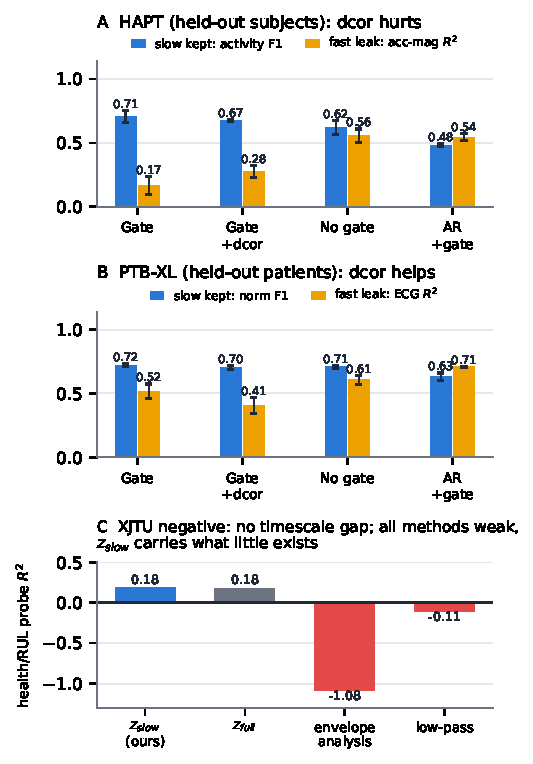
\includegraphics[width=.92\linewidth]{fig_real.pdf}
\vspace{-4mm}
\caption{\small \textbf{Real data (3 seeds).} Gate and gate+dcor shown on
both datasets: dcor hurts HAPT (\textbf{A}), helps PTB-XL (\textbf{B}).
\textbf{C:} XJTU, the predicted negative --- no timescale gap; classical
envelope features fail to transfer across bearings.}
\vspace{-3mm}
\end{figure}

\section{Limitations and future work}
\textbf{Limitations.} Exclusion is soft and \emph{linear-level}: nonlinear
probes recover more of the fast factor than linear ones (MLP $R^2$ $0.45$
vs.\ $0.19$), which is exactly the boundary Prop.~2 identifies --- our claim
is linear-subspace separation, not information-theoretic removal. Gated
training has a downstream cost on some data (HAPT: full embedding
$0.80\!\to\!0.76$ F1; $z^{\mathrm{slow}}$ alone $0.71$), compensated by
robustness and selective use (on synthetic, $z^{\mathrm{slow}}$ \emph{beats}
the full embedding). The dcor polarity is data-dependent and not yet
decidable label-free; $\tau$ is label-free but
$d_{\mathrm{slow}},\lambda$ are not. The design assumes exactly two
timescales, and $\tau=c\,T_{\mathrm{ac}}$ assumes fast dynamics dominate the
ACF. Training is fully label-free; validation, as standard in
disentanglement, is not.
\textbf{Future work (in progress or planned).} Unsupervised model selection
(a health-metric criterion currently rejects broken configurations but
cannot fine-tune); anomaly attribution via horizon-split residuals (point
detection works in a pilot; contextual detection needs novelty-sensitive
machinery); additional datasets with pre-registered gap screening (Sleep-EDF
\cite{kemp2000analysis}, C-MAPSS \cite{saxena2008damage}); external
self-supervised baselines (TS2Vec \cite{yue2022ts2vec}, masked
reconstruction); a nonlinear (HSIC) dependence penalty targeting the
linear-level limitation.

{\footnotesize
\begin{thebibliography}{99}\setlength{\itemsep}{0pt}
\bibitem{wiskott2002slow} L. Wiskott, T. Sejnowski. Slow feature analysis.
\emph{Neural Comp.}, 2002.
\bibitem{bialek2001predictability} W. Bialek, I. Nemenman, N. Tishby.
Predictability, complexity, and learning. \emph{Neural Comp.}, 2001.
\bibitem{creutzig2009past} F. Creutzig, A. Globerson, N. Tishby. Past-future
information bottleneck in dynamical systems. \emph{Phys.\ Rev.\ E}, 2009.
\bibitem{hyvarinen2016unsupervised} A. Hyv\"arinen, H. Morioka.
Time-contrastive learning and nonlinear ICA. \emph{NeurIPS}, 2016.
\bibitem{klindt2021towards} D. Klindt et al. Towards nonlinear disentanglement
in natural data with temporal sparse coding. \emph{ICLR}, 2021.
\bibitem{locatello2019challenging} F. Locatello et al. Challenging common
assumptions in unsupervised disentanglement. \emph{ICML}, 2019.
\bibitem{hsu2017unsupervised} W.-N. Hsu, Y. Zhang, J. Glass. Disentangled
representations from sequential data. \emph{NeurIPS}, 2017.
\bibitem{bai2021contrastively} J. Bai, W. Wang, C. Gomes. Contrastively
disentangled sequential VAE. \emph{NeurIPS}, 2021.
\bibitem{oord2018representation} A. van den Oord, Y. Li, O. Vinyals.
Contrastive predictive coding. arXiv:1807.03748, 2018.
\bibitem{assran2023self} M. Assran et al. I-JEPA. \emph{CVPR}, 2023.
\bibitem{baevski2022data2vec} A. Baevski et al. data2vec. \emph{ICML}, 2022.
\bibitem{hepa2026} HEPA: horizon-conditioned joint-embedding prediction for
time series. 2026.
\bibitem{bardes2022vicreg} A. Bardes, J. Ponce, Y. LeCun. VICReg. \emph{ICLR},
2022.
\bibitem{garrido2023rankme} Q. Garrido et al. RankMe. \emph{ICML}, 2023.
\bibitem{yue2022ts2vec} Z. Yue et al. TS2Vec. \emph{AAAI}, 2022.
\bibitem{mallat1999wavelet} S. Mallat. \emph{A Wavelet Tour of Signal
Processing}. Academic Press, 1999.
\bibitem{huang1998empirical} N. E. Huang et al. Empirical mode decomposition.
\emph{Proc.\ R.\ Soc.\ A}, 1998.
\bibitem{randall2011rolling} R. B. Randall, J. Antoni. Rolling element bearing
diagnostics. \emph{MSSP}, 2011.
\bibitem{reyes2016transition} J.-L. Reyes-Ortiz et al. Transition-aware human
activity recognition (HAPT). \emph{Neurocomputing}, 2016.
\bibitem{wagner2020ptb} P. Wagner et al. PTB-XL. \emph{Scientific Data}, 2020.
\bibitem{wang2020xjtu} B. Wang et al. XJTU-SY bearing datasets. \emph{IEEE
Trans.\ Reliability}, 2020.
\bibitem{saxena2008damage} A. Saxena et al. C-MAPSS run-to-failure simulation.
\emph{PHM}, 2008.
\bibitem{kemp2000analysis} B. Kemp et al. Sleep-EDF. \emph{IEEE Trans.\
Biomed.\ Eng.}, 2000.
\end{thebibliography}
}

\end{document}
